% !TeX root=main.tex
\chapter{تعاریف و مفاهیم مبنایی}
\thispagestyle{empty}
	همان‌طور که قبلاً اشاره شد مسئله پرسش و پاسخ تصویری در تقاطع دو حوزه پردازش زبان طبیعی و بینایی ماشین قرار می‌گیرد. از این رو قبل از بررسی کارهای مرتبط با مسئله پرسش و پاسخ تصویری، نیاز است تا با مفاهیم مربوط به این دو حوزه آشنا شویم. در ادامه این فصل به شرح مفاهیم و تعاریف پایه می‌پردازیم.

\section{پردازش زبان طبیعی}
	پردازش زبان‌ طبیعی 
	\footnote{\lr{Natural Language Processing}}
	یکی از زیرشاخه‌های علوم کامپیوتر و هوش مصنوعی است که به تعامل بین کامپیوتر و زبان‌های (طبیعی) انسانی می‌پردازد. هدف اصلی در پردازش زبان طبیعی، تحلیل زبانهای طبیعی به منظور آسان‌تر ساختن فهم آ‌ن‌ها برای کامپیوتر می‌باشد. مسلماً درصورتی که کامپیوتر بتواند توسط زبان‌های طبیعی با انسان ارتباط برقرار کند، بسیاری از مشکلات تعامل انسان با کامپیوتر حل شده و زندگی برای انسان‌ها راحت‌تر خواهد شد. با پیشرفت تکنولوژی و بوجود آمدن نیازهای متفاوت برای انسان‌ها، کاربردهای جدیدی برای این حوزه تعریف می‌شود. ترجمه ماشینی، خلاصه‌سازی متون، تحلیل احساسات، طبقه‌بندی متون، سیستم‌های توصیه‌گر، غلط‌یابی متون و ... از جمله مهم‌ترین کاربردهای پردازش زبان طبیعی است.
	
\section{بینایی ماشین}
 بینایی ماشین
	\footnote{\lr{Computer Vision}}
  جز حوزه‌های در حال توسعه در علوم کامپیوتر و هوش مصنوعی محسوب می‌شود که سعی دارد از طریق پردازش تصاویر دوبعدی، جهان سه بعدی پیرامون را بازسازی و تفسیر کند. به بیان ساده، بینایی ماشین یعنی کامپیوترها بتوانند جهان را به کمک دوربین‌ها ببینند، بفهمند و حتی از بینایی انسان پیشی بگیرند. بینایی کامپیوتر دارای کاربردهای بسیار متنوعی مانند طبقه‌بندی اشیا، تشخیص اشیا، تقسیم‌بندی اشیا، تشخیص چهره و ... است.

\section{یادگیری عمیق}
	یادگیری عمیق
	\footnote{\lr{deep learning}}
	زیر شاخه‌ای از یادگیری ماشین
	 \footnote{\lr{machine learning}}
	  است که تلاش می‌کند تا مفاهیم انتزاعی سطح بالا را با استفاده از نمونه‌های(دادگان) زیاد مدل نماید. بیشتر روش‌های یادگیری عمیق از معماری شبکه‌های عصبی مصنوعی
	  \footnote{\lr{artificial neural networks}}
	  استفاده می‌کنند‌. به همین دلیل است که اغلب از مدل‌های یادگیری عمیق به عنوان شبکه‌های عصبی عمیق یاد می‌شود. اصطلاح «عمیق» معمولاً به تعداد لایه‌های پنهان در شبکه عصبی اشاره دارد. شبکه‌های عصبی سنتی فقط شامل 2 یا 3 لایه پنهان هستند، در حالی که شبکه‌های عمیق می‌توانند تا 150 لایه داشته باشند. مدل های یادگیری عمیق معمولا با استفاده از مجموعه‌های بزرگی از داده‌های دارای برچسب و معماری شبکه عصبی که ویژگی‌ها را مستقیماً از داده‌ها بدون نیاز به استخراج دستی ویژگی‌ها یاد می‌گیرند، آموزش می‌بینند.
	  
	  در حالی که یادگیری عمیق برای اولین بار در دهه 1980 مطرح شد اما به دلیل تولید داده‌های زیاد، افزایش  قدرت محاسباتی و پیشرفت الگوریتم‌های این حوزه شاهد پیشرفت چشمگیر یادگیری عمیق در سال‌های اخیر هستیم. در حال حاضر شبکه‌های عصبی عمیق در حوزه‌های زیادی از جمله پردازش زبان طبیعی، بینایی ماشین، پردازش گفتار و... کاربرد دارد. شبکه‌های عصبی کانولوشنی و شبکه‌های عصبی بازگشتی از مهم‌ترین و پرکاربردترین شبکه‌های یادگیری عمیق هستند.
	\begin{figure}
	  	\center{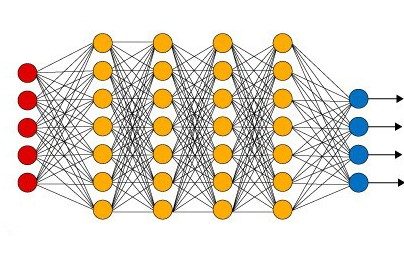
\includegraphics[scale=0.5]{images/DNN.jpg}}
	  	\caption[نمونه‌ای از شبکه عصبی عمیق]{نمونه‌ای از شبکه عصبی عمیق. نورون‌های قرمز لایه‌ی ورودی ، نورون‌های نارنجی لایه‌ی مخفی و نورون‌های آبی لایه‌ی خروجی را نشان ‌می‌دهند.}
	  	\label{fig:DNN}
	\end{figure}

\section{شبکه‌های عصبی کانولوشنی}
	شبکه‌های عصبی کانولوشنی
	\footnote{\lr{convolutional neural networks}}
	دسته‌ای از شبکه‌های عصبی عمیق هستند که معمولاً برای تجزیه و تحلیل تصاویر استفاده می‌شوند. برخلاف شبکه‌های کاملاً متصل که هر نورون در یک لایه به همه نورون‌های لایه بعدی متصل است، در شبکه‌های عصبی کانولوشنی هر نورون تنها به بخشی از نورون‌های لایه‌ی بعدی متصل است. این خاصیت به دلیل انجام عملیات کانولوشن در شبکه‌های عصبی کانولوشنی است و باعث می‌شود که الگوهای محلی را از داده فرا بگیرند. در حالی که شبکه‌های کاملاً متصل الگوهای سراسری را یاد می‌گیرند. معمولا از شبکه‌های عصبی کانولوشنی برای استخراج ویژگی از تصویر استفاده می‌شود. در ادامه چند نمونه از برجسته‌ترین شبکه‌های عصبی کانولوشنی را معرفی ‌می‌کنیم.
	\begin{table}
		\caption{مقایسه مهم‌ترین شبکه‌های عصبی کانولوشنی آموزش‌دیده بر روی مجموعه‌داده \lr{ImageNet}}
		\label{tabel:2}
		\begin{center}
			\begin{tabular}{ |c|c|c|c|c|c| } 
				\hline
				\textbf{مدل \lr{CNN}} & \textbf{سال} & \textbf{تعداد لایه‌‌ها} & \textbf{ابعاد ورودی}  & \textbf{ابعاد خروجی} &
				\textbf{پارامترها}  \\
				\hline \hline
				\textbf{\lr{AlexNet}\cite{hinton2012imagenet}} & 2012 & 8 & 227×227 & 4096 & 60میلیون  \\
				\hline
				\textbf{\lr{VGGNet}\cite{simonyan2014very}} & 2014 & 19 & 224×224 & 4096 & 138میلیون \\
				\hline
				\textbf{\lr{GoogleNet}\cite{szegedy2015going}} & 2014 & 22 & 229×229 & 1024 & 5میلیون \\
				\hline
				\textbf{\lr{ResNet}\cite{he2016deep}} & 2015 & 152 & 224×224 & 20148 & 26میلیون\\
				\hline
			\end{tabular}
		\end{center}
	\end{table}

\subsection{\lr{AlexNet}}
	\begin{figure}
		\center{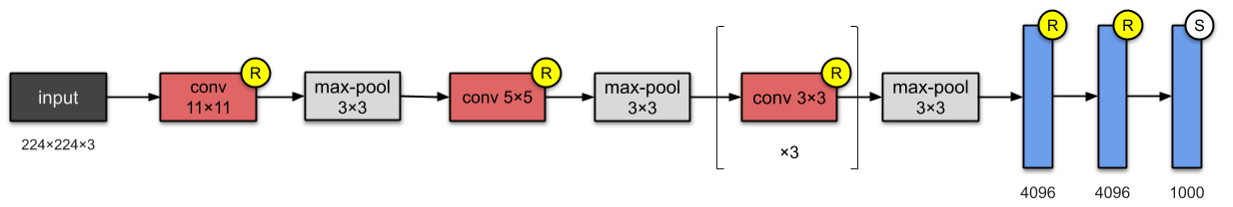
\includegraphics[scale=0.4]{images/AlexNet.png}}
		\caption[معماری شبکه \lr{AlexNet}]{معماری شبکه
			\href{https://towardsdatascience.com/illustrated-10-cnn-architectures-95d78ace614d\#e971}{\lr{AlexNet}}}
		\label{fig:AlexNet}
	\end{figure}
	در سال 2012، 
		\lr{AlexNet}
	 به طور قابل توجهی بهتر از تمام رقبای قبلی عمل کرد. در این شبکه از 5 لایه‌ی کانولوشنی و 3 لایه‌ی کاملاً متصل استفاده شده است. معماری این شبکه در شکل 
	 \ref{fig:AlexNet}
	 نمایش داده شده است.

\subsection{\lr{VGGNet}}
	\begin{figure}
		\center{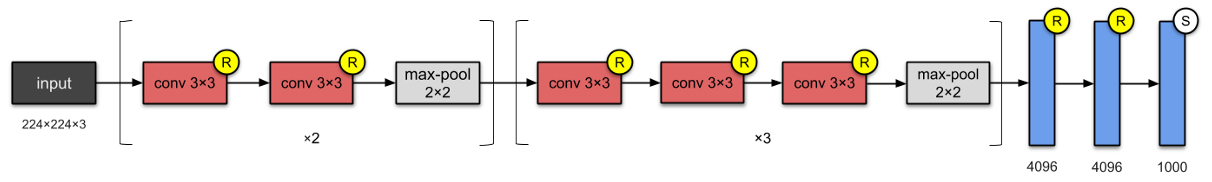
\includegraphics[scale=0.4]{images/VGGNet.png}}
		\caption[معماری شبکه \lr{VGGNet}]{معماری شبکه 
			\href{https://towardsdatascience.com/illustrated-10-cnn-architectures-95d78ace614d\#c5a6}{\lr{VGGNet}}}
		\label{fig:VGGNet}
	\end{figure}
	شبکه 
	\lr{VGGNet}
	در سال 2014 معرفی شد. شبکه
	\lr{VGGNet}
	 از 16 لایه کانولوشن تشکیل شده است و معماری بسیار یکنواختی دارد. شبکه
	 \lr{VGGNet}
	 یکی از محبوب‌ترین شبکه‌ها برای استخراج ویژگی است. تعداد پارامترهای این شبکه برابر با 138 میلیون است.  معماری این شبکه در شکل 
	 \ref{fig:VGGNet}
	 نشان داده شده است.
 
\subsection{\lr{GoogleNet}}
	\begin{figure}
		\center{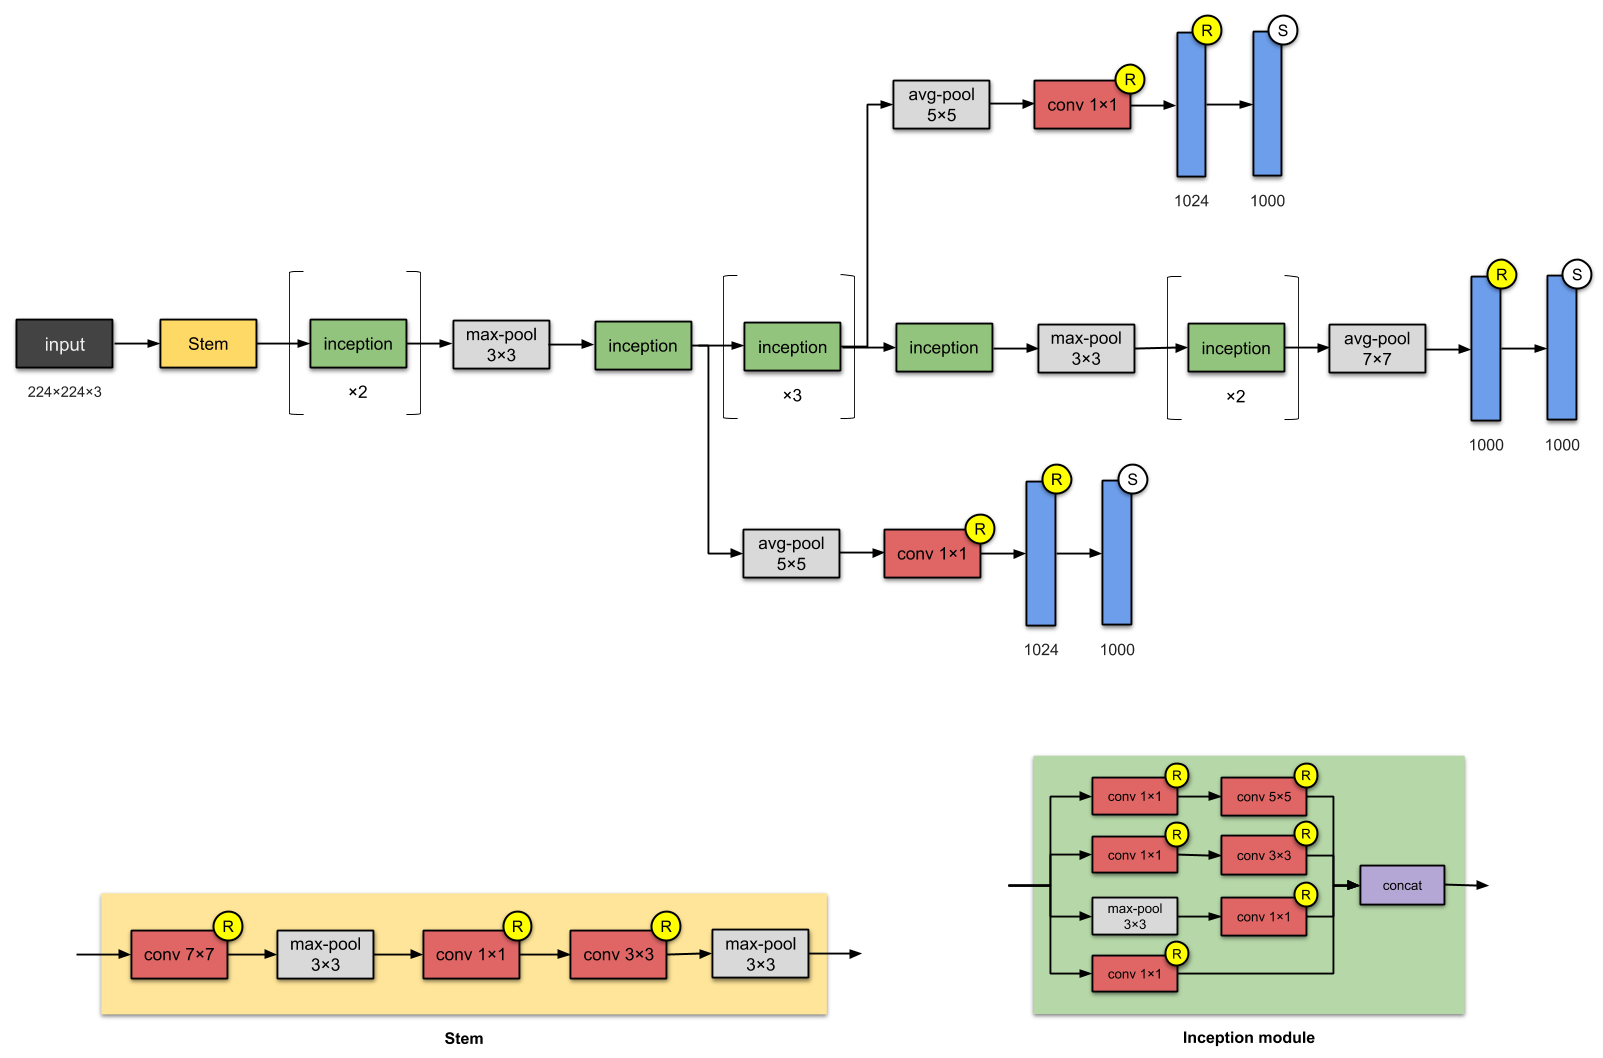
\includegraphics[scale=0.3]{images/GoogleNet.png}}
		\caption[معماری شبکه \lr{GoogleNet}]{معماری شبکه
			\href{https://towardsdatascience.com/illustrated-10-cnn-architectures-95d78ace614d\#81e0}{\lr{GoogleNet}}}
		\label{fig:GoogleNet}
	\end{figure}
	شبکه
	\lr{GoogleNet}
	همزمان با شبکه 
	\lr{VGGNet}
	در سال 2014 معرفی شد و  توانست بر شبکه
	\lr{VGGNet}  
	غلبه کند و دقت بالاتری را بر روی مجموعه داده
	\lr{ImageNet}
	بدست آورد. مهم‌ترین علت موفقیت آن استفاده از ماژول
	\lr{inception}
	بود که منجر به کاهش شدید تعداد پارامترها در این شبکه شد. شبکه
	\lr{GoogleNet}
	از 22 لایه با 4 میلیون پارامتر تشکیل شده است. معماری این شبکه در شکل 
	\ref{fig:GoogleNet}
	نمایش داده شده است.

\subsection{\lr{ResNet}}
	\begin{figure}
		\center{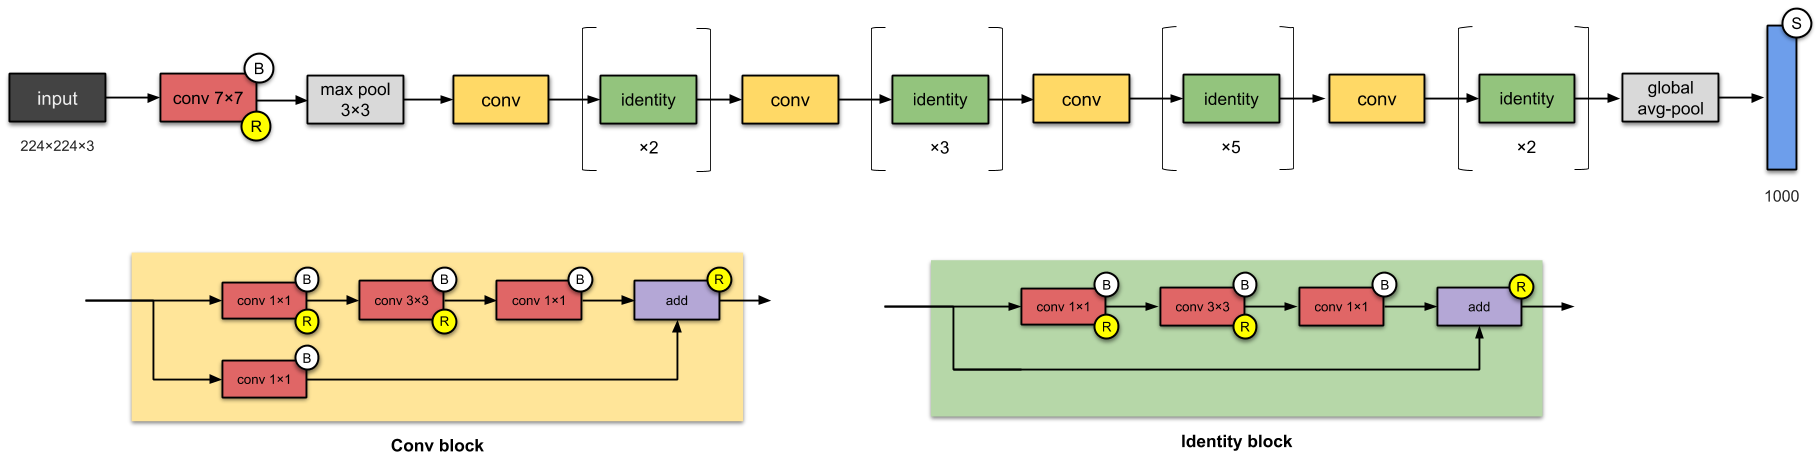
\includegraphics[scale=0.3]{images/ResNet.png}}
		\caption[معماری شبکه \lr{ResNet}]{معماری شبکه 
			\href{https://towardsdatascience.com/illustrated-10-cnn-architectures-95d78ace614d\#e4b1}{\lr{ResNet}}}
		\label{fig:ResNet}
	\end{figure}
	شبکه
	\lr{ResNet}
	با معرفی مفهوم جدید
	\lr{skip connection]}
	این امکان را برای شبکه‌های عصبی کانولوشنی ایجاد کرد که شبکه‌ها عمیق‌تر شوند و در عین حال آموزش در زمان کمتری انجام شود. با وجود اتصالات 
	\lr{skip conection}
	ورودی هر لایه بدون واسطه به لایه بعدی منتقل می‌شود بنابراین مشکل از بین رفتن گرادیان در شبکه‌های عمیق رفع می‌شود. 152 لایه در شبکه 
	\lr{ResNet}
	به کار رفته است. معماری این شبکه در شکل 
	\ref{fig:ResNet}
	نشان داده شده است.

\section{شبکه‌های عصبی بازگشتی}
	شبکه‌های عصبی بازگشتی
	\footnote{\lr{recurrent neural networks}}
	دسته‌ی دیگری از شبکه‌های عصبی عمیق هستند که معمولا برای پردازش داده‌های دنباله‌دار مانند جملات، صوت و ویدئو استفاده می‌شوند. این شبکه‌ها دارای یک نوع حافظه هستند که اطلاعاتی تا کنون دیده‌اند را ضبط می‌کنند. در تئوری این‌طور به نظر می‌رسد که شبکه‌های عصبی بازگشتی می‌توانند اطلاعات موجود در یک دنباله طولانی را ضبط و از آن‌ها استفاده کنند اما در عمل این‌طور نیست و بسیار محدود هستند ‌و فقط اطلاعات چند گام قبل را نگه می‌دارند. شبکه‌های عصبی بازگشتی پارامترهای مشابهی را بین همه گام‌های زمانی به اشتراک می‌گذارند . این بدین معنی است که در هر گام زمانی عملیات مشابهی را انجام می‌دهند و فقط ورودی‌ها متفاوت هستند. با این تکنیک تعداد کلی پارامتر‌هایی که شبکه باید یاد بگیرد به شدت کاهش پیدا می‌کند. در ادامه این بخش به معرفی دو شبکه عصبی بازگشتی معروف می‌پردازیم.
	
\subsection{\lr{LSTM}}
	مدل 
	\lr{LSTM} \footnote{\lr{Long Short-Term Memory}}
	در سال 1995 برای توسعه شبکه‌های عصبی بازگشتی ظهور پیدا کرد. شبکه 
	\lr{LSTM}
	برای حل مشکل  ناپدید شدن گرادیان در شبکه‌های عصبی بازگشتی بوجود آمد. بزرگ‌ترین ویژگی 
	\lr{LSTM}
	 امکان یادگیری وابستگی بلند مدت است که توسط شبکه‌های عصبی بازگشتی امکان‌پذیر نبود. برای پیش‌بینی گام زمانی بعدی نیاز است که مقادیر وزن‌ها در شبکه بروزرسانی شوند که این کار مستلزم حفظ اطلاعات گام‌های زمانی ابتدایی است. یک شبکه عصبی بازگشتی فقط می‌تواند تعداد محدودی از وابستگی‌های کوتاه مدت را یاد بگیرد ، اما سری‌های زمانی بلند مدت قایل یادگیری توسط شبکه‌های عصبی بازگشتی نیستند اما 
	\lr{LSTM}
	 می‌تواند این وابستگی‌های بلند مدت را به درستی یاد بگیرند.
	 
\subsection{\lr{GRU}}
	یکی دیگر از شبکه‌های عصبی بازگشتی، 
	\lr{GRU}\footnote{\lr{Gated Recurrent Unit}}
	است که در سال 2014 معرفی شد. این شبکه نیز مانند 
	\lr{LSTM}
	مشکل ناپدیدشدن گرادیان در شبکه‌های عصبی بازگشتی را حل می‌کند. در واقع 
	\lr{GRU}
	نوع خاصی از 
	\lr{LSTM}
	است که با کم کردن تعداد دروازه‌ها، سرعت محاسبات را افزایش داده است.
	 \begin{figure}
	 	\center{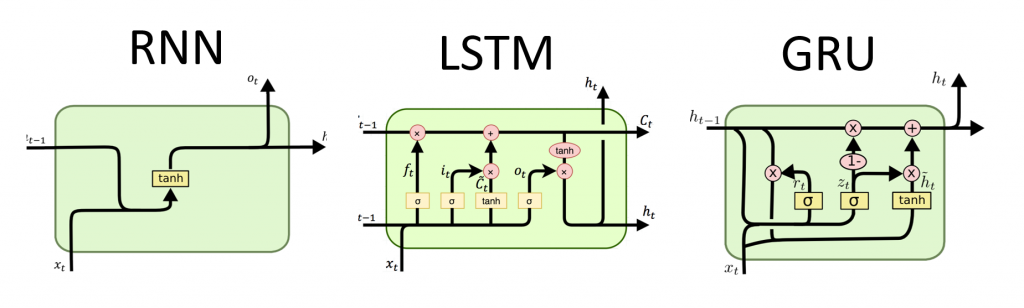
\includegraphics[scale=0.5]{images/RNN-LSTM-GRU.png}}
	 	\caption[مقایسه معماری شبکه‌‌های عصبی بازگشتی، \lr{LSTM} و \lr{GRU}]{مقایسه معماری شبکه‌‌های عصبی بازگشتی، \lr{LSTM} و \lr{GRU} \href{http://dprogrammer.org/rnn-lstm-gru}{[منبع]}}
	 	\label{fig:RNN-LSTM-GRU}
	 \end{figure}

\section{تعبیه کلمات}
	بیشتر الگوریتم‌های یادگیری ماشین و یادگیری عمیق  قادر به پردازش متن به شکل خام وساده نیستند  و برای بازنمایی متن‌ها نیاز به تعبیه کلمات 
	\footnote{\lr{word embedding}}
	دارند. تعبیه کلمات نگاشت کلمات یا عبارات از واژگان به بردارهای عددی است تا کامپیوترها بتوانند به راحتی آن‌ها را پردازش کنند. تعبیه کلمات عمدتاً برای مدل‌سازی زبان و یادگیری ویژگی در پردازش زبان طبیعی استفاده می‌شود. ایده اصلی در پشت تمام روش‌های تعبیه کلمات، گرفتن هرچه بیشتر اطلاعات معنایی و ریخت‌شناسی است. روش‌های تعبیه کلمات بسیاری در مسئله پرسش و پاسخ تصویری استفاده شده است. در ادامه به برجسته‌ترین و پرکاربردترین روش‌های تعبیه کلمات موجود و استفاده‌شده در مسئله پرسش و پاسخ تصویری می‌پردازیم و معایب و مزایای هر کدام را بررسی خواهیم کرد.
\subsection{کدگذاری \lr{one-hot}}
	روش کدگذاری
	\lr{one-hot}
	ساده‌ترین روش تعبیه کلمات است. در این روش یک لغت‌‌نامه از همه واژه‌های منحصربه‌فرد موجود در مجموعه‌داده ساخته‌می‌شود و اندیس یکتایی به هر واژه اختصاص می‌یابد. بنابراین برای هر واژه یک بردار به طول تعداد واژ‌ه‌ها ساخته می‌شود که تمامی مقادیر آن صفر است به جز اندیس مربوط به همان واژه که مقدار آن یک است. پیاده‌سازی این روش آسان است اما طول بردارها  بزرگ است زیرا برابر با تعداد کل واژه‌های منحصر به فرد مجموعه داده است و هزینه زیادی برای ذخیره‌سازی دارد. بزرگترین عیب این روش  این است که نمی‌توان از آن معنا  و مفهوم استخراج کرد زیرا فاصله‌ی تمامی کلمات با هم یکسان است. در صورتی که ما انتظار داریم؛ کلماتی که مشابه هم هستند بردارهای نزدیک به هم یا مشابه هم داشته باشند و کلملاتی که معنای متفاوتی با یکدیگر دارند تا حد امکان بردارهایشان از هم دور باشند. 

\subsection{\lr{CBOW}‌ و \lr{Skip-gram}}
	برای رفع مشکلات کدگذاری 
	\lr{one-hot}
	، دو روش
	\lr{CBOW} 
	\footnote{\lr{Continouse Bag Of Words}}
	\cite{mikolov2013efficient}
	و
	\lr{Skip-gram}
	\cite{mikolov2013efficient}
	پیشنهاد شد که از شبکه‌های عصبی به عنوان جز اصلی خود استفاده می‌کنند. این دو مدل بر عکس هم کار می‌کنند.	در هر دو مدل، از یک شبکه عصبی سه لایه که شامل لایه ورودی، لایه پنهان ولایه خروجی است، استفاده شده است. درمدل 
	\lr{CBOW} 
	کلمات اطراف و نزدیک به یک کلمه(\lr{n-1}کلمه) به لایه ورودی داده می‌شود و مدل سعی می‌کند این کلمه (\lr{n}امین کلمه) را حدس بزند.  بعد از آموزش این شبکه‌، وزن بین لایه‌ی پنهان و لایه خروجی، کلمات مجموعه داده را بازنمایی می‌کند که هر ستون آن بردار مربوط به یک کلمه را نشان می‌دهد. در مدل
	\lr{skip-gram}
	برعکس 
	\lr{CBOW} 
	یک کلمه به شبکه ورودی داده می‌شود و شبکه باید کلمات اطراف و نزدیک به آن را حدس بزند. 
	\begin{figure}
		\center{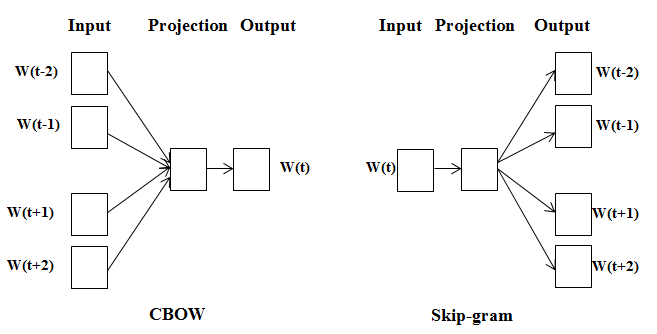
\includegraphics[scale=0.5]{images/2.png}}
		\caption{
			معماری شبکه 
			\lr{CBOW}
			و
			\lr{Skip-gram}	
		}
		\label{fig:CBOW&skip-gram}
	\end{figure}
	معماری 
	\lr{CBOW}
	و
	\lr{Skip-gram}
	در شکل 
	\ref{fig:CBOW&skip-gram}
	آورده شده است. 

\subsection{\lr{GloVe}}
	یکی دیگر از تعبیه کلمات مشهور، مدل بردار سراسری یا به اختصار 
	\lr{GloVe}
	\footnote{\lr{Global Vector}}
	است که توسط پنینگتون و همکاران 
	\cite{pennington2014glove}
	در سال 2014 در تیم پردازش زبان‌های طبیعی دانشگاه استنفورد معرفی و توسعه داده شد. در 
	\lr{GloVe}
	فاصله میان بردار‌ها نشان‌دهنده شباهت معنایی میان آن بردارها است.
	
\subsection{\lr{CNN}‌، \lr{LSTM}‌‌و \lr{GRU}}
	با پیشرفت یادگیری عمیق در دهه اخیر، محققان برای استخراج ویژگی و بازنمایی متن از
	\lr{CNN}
	،
	\lr{LSTM}
	\cite{hochreiter1997long}
	و
	\lr{GRU}
	\cite{cho2014learning}
	استفاده می‌کنند. برای استخراج ویژگی از متن با استفاده از 
	\lr{CNN}
	بردارهای کلمات در کنار هم قرار داده می‌شود سپس به لایه‌های کانولوشنی یک بعدی داده می‌شود و فیلتر‌های متفاوتی بر روی آن‌ها اعمال می‌شود و پس از عبور از لایه‌ 
	\lr{max-pooling}
	ویژگی‌ها بدست می‌آید. همچنین برای استخراج ویژگی از متن با استفاده از 
	\lr{LSTM}
	و
	\lr{GRU}
	کافی است، بردار کلمات یک جمله به عنوان ورودی به این لایه‌ها داده شود.سپس خروجی آخرین گام زمانی به عنوان ویژگی کل جمله خواهد بود. 
